\def\year{2018}\relax
%File: formatting-instruction.tex
\documentclass[letterpaper]{article}
\usepackage{aaai18}
\usepackage{times}
\usepackage{helvet}
\usepackage{courier}
\usepackage{url}  %Required
\usepackage{graphicx}  %Required
\frenchspacing
\setlength{\pdfpagewidth}{8.5in}
\setlength{\pdfpageheight}{11in}
\usepackage{amsthm,amsfonts,amssymb,amsmath}
\usepackage{array}
\usepackage{color}
\usepackage{colortbl}
\usepackage{graphicx} 
\usepackage{calc}
\usepackage{mathtools}
\usepackage{tikz}
\usetikzlibrary{arrows,shapes,trees}
\DeclareMathOperator*{\argmax}{arg\,max}
\DeclareMathOperator*{\argmin}{arg\,min}
\DeclarePairedDelimiter{\norma}{\lVert}{\rVert}
 \theoremstyle{plain}
\newtheorem{theorem}{Theorem}[section]
\newtheorem{lemma}{Lemma}[section]
\newtheorem{corollary}{Corollary}[section]
\theoremstyle{definition} 
\newtheorem{definition}{Definition}[section]
\theoremstyle{remark} 
\newtheorem{observation}{Observation}
\theoremstyle{definition}
\newtheorem{example}{Example}[section]
\usepackage{listings}
\lstset{
  language=Prolog,
  aboveskip=1mm,
  belowskip=1mm,
  showstringspaces=false,
  columns=flexible,
  %numbers=none,
  % basicstyle={\ttfamily},
 basicstyle={\footnotesize\ttfamily},
  breaklines=false,
  breakatwhitespace=true,
  tabsize=3
}
\def\mcode#1{\lstinline[mathescape=true]{#1}}
\pdfinfo{
/Title (Properties of Probabilistic Concurrent Constraint Programs)
/Author (Vijay Saraswat, Cristina Cornelio, Radha Jagadeesan)}
\setcounter{secnumdepth}{0}  
\frenchspacing
 \begin{document}
% The file aaai.sty is the style file for AAAI Press 
% proceedings, working notes, and technical reports.
%


%full-length papers: 6 pages + 1 page for references in AAAI format


\title{Properties of Probabilistic Concurrent Constraint Programs}
\author{Vijay Saraswat \and Cristina Cornelio\\
IBM T.J. Watson Research Center \\
Yorktown Heights, New York, U.S.\\
ccornel@us.ibm.com, vijay@saraswat.org\\
\And
Radha Jagadeesan\\
DePaul University\\
243 S. Wabash Avenue\\
Chicago, Illinois 60604-2287\\
rjagadeesan@cs.depaul.edu 
}
\maketitle
\begin{abstract}
The Probabilistic Concurrent Constraint (pcc) programming framework was introduced in 1997 by adding just a sampling agent $X\sim pd$ in concurrent constraint programming (ccp) languages. Unlike subsequent probabilistic programming frameworks, no ``observe'' capability needs to be added since it is already present in the framework through the (\(tell\)) \(c\) operator. For the application programmer, pcc provides a powerful compositional, logical framework in which sophisticated joint probability distributions can be defined by using constraints to conditionally rule out portions of the search space.

The underlying ccp framework enjoys many logical properties, related to the interpretation of ccp agents as closure operators over the underlying constraint system.  For instance, if an agent $A$ produces an answer constraint $c$, and $c$ entails $d$, then the agent $(A,d)$ will also produce the answer $c$. This paper shows how such logical properties carry over to pcc, and how they relate to the interpretation of pcc as a probabilistic framework. In particular we show how conditional probability distributions can be represented in pcc, and how marginalization is related to existential quantification.  Additionally, we show how many probabilistic programming idioms can be represented in pcc.

These results provide a foundation for the practical use of pcc as a probabilistic programming language.
\end{abstract}

\usepackage{relsize}
\usepackage{amsmath}
\usepackage{url}

\usepackage{listings}

%\usepackage{color}
%
%\definecolor{Brown}{cmyk}{0,0.49,0.71,0.37}
%\definecolor{RoyalBlue}{cmyk}{0.71,0.53,0,0.12}
%\definecolor{OliveGreen}{cmyk}{0.64,0,0.95,0.40}
%\definecolor{Red}{cmyk}{0,0.80,0.80,0.10}
%\definecolor{Gray}{cmyk}{0.2,0.2,0.2,0.2}
%\definecolor{Black}{cmyk}{0,0,0,1}
\lstdefinelanguage{X10}%
  {morekeywords={abstract,break,case,catch,class,%
      const,continue,default,do,else,extends,false,final,%
      finally,for,goto,if,implements,import,instanceof,%
      interface,label,native,new,null,package,private,protected,%
      public,return,static,super,switch,synchronized,this,throw,%
      throws,transient,true,try,volatile,while,%
      async,atomic,when,foreach,ateach,finish,clocked,%
      type,here,%
      self,property,%
      future,to,has,as,var,val,def,where,in,%
      next,value,or,await,current,any},%
   basicstyle=\normalfont\ttfamily,%\color{Red},%
   keywordstyle=\bf\ttfamily,%\color{OliveGreen},%
   commentstyle=\normalfont\ttfamily,%\color{Gray},%
   identifierstyle=\normalfont\ttfamily,%\color{Red},%
   stringstyle=\normalfont\ttfamily,%
   tabsize=4,%
   showstringspaces=false,%
   sensitive,%
   morecomment=[l]//,%
   morecomment=[s]{/*}{*/},%
   morestring=[b]",%
   morestring=[b]',%
   columns=fullflexible,%
   mathescape=false,%
   keepspaces=true,%
   showlines=false,%
   breaklines=true,%
   breakatwhitespace=true,%
   postbreak={},%
   %breakautoindent=true,%
   %breakindent=0pt,%
   %prebreak={},%
  }

\lstnewenvironment{xtenmath}
  {\lstset{language=X10,breaklines=false,captionpos=b,xleftmargin=2em,mathescape=true}}
  {}

\lstnewenvironment{xten}
  {\lstset{language=X10,breaklines=false,captionpos=b}} %,xleftmargin=2em
  {}

%{numbers=left, numberstyle=\tiny, stepnumber=2, numbersep=5pt
% numbers=left,
\lstset{language=x10,basicstyle=\ttfamily\small}
%\lstset{language=java,basicstyle=\ttfamily\small}


\usepackage{algorithm} % [plain]
\usepackage{algorithmic} % [noend]
\renewcommand\algorithmiccomment[1]{// \textit{#1}} %



% For fancy end of line formatting.
\usepackage{microtype}


% For smaller font.
\usepackage{pslatex}


\usepackage{xspace}
\usepackage{../yglabels}
\usepackage{../yglang}
\usepackage{../ygequation}
\usepackage{graphicx}
%\usepackage{epstopdf}

\newcommand{\formalrule}[1]{\mbox{\textsc{\scriptsize #1}}}
\newcommand{\myrule}[2]{\textbf{Rule #1:} #2.}
%\newcommand{\myrule}[1]{\textsc{\codesmaller #1 Rule}}
\newcommand{\umyrule}[1]{\textbf{\underline{\textsc{\codesmaller #1 Rule}}}}


% \small \footnotesize \scriptsize \tiny
% \codesize and \scriptsize seem to do the same thing.
% \newcommand{\code}[1]{\texttt{\textup{\footnotesize #1}}}
% \newcommand{\code}[1]{\texttt{\textup{\codesize #1}}}
\newcommand{\normalcode}[1]{\texttt{\textup{#1}}}
\def\codesmaller{\small}
\newcommand{\myCOMMENT}[1]{\COMMENT{\small #1}}
\newcommand{\code}[1]{\texttt{\textup{\codesmaller #1}}}
% \newcommand{\code}[1]{\ifmmode{\mbox{\smaller\ttfamily{#1}}}
%                       \else{\smaller\ttfamily #1}\fi}
\newcommand{\smallcode}[1]{\texttt{\textup{\scriptsize #1}}}
%\newcommand{\myparagraph}[1]{\noindent\textit{\textbf{#1}}~} %\vspace{-1mm}\paragraph{#1}}

% See: \usepackage{bold-extra} if you want to do \textbf
\newcommand{\keyword}[1]{\code{#1}}

% For new, method invocation, and cast:
\newcommand{\hparen}[1]{\code{(}#1\code{)}}

\newcommand{\hgn}[1]{\lt#1\gt} % type parameters and generic method parameters

\newcommand{\Own}{{\it O}}
\newcommand{\Ifn}[1]{\ensuremath{I(#1)}}
\newcommand{\Ofn}[1]{\ensuremath{O(#1)}}
\newcommand{\Cooker}[1]{\ensuremath{{\kappa}(#1)}}
\newcommand{\Owner}[1]{\ensuremath{{\theta}(#1)}}
\newcommand{\Oprec}[0]{\ensuremath{\preceq_{\theta}}}
\newcommand{\Tprec}[0]{\ensuremath{\preceq^T}}
\newcommand{\TprecNotEqual}[0]{\ensuremath{\prec^T}}
\newcommand{\OprecNotEqual}[0]{\ensuremath{\prec_{\theta}}}
\newcommand{\IfnDelta}[1]{\ensuremath{I_\Delta(#1)}}
\newcommand\Abs[1]{\ensuremath{\left\lvert#1\right\rvert}}
\newcommand{\erase}[1]{\ensuremath{\Abs{#1}}}

\newcommand{\CookerH}[1]{\ensuremath{{\kappa}_H(#1)}}
\newcommand{\IfnH}[1]{\ensuremath{I_H(#1)}}
\newcommand{\OwnerH}[1]{\ensuremath{{\theta}_H(#1)}}
\newcommand{\Gdash}[0]{\ensuremath{\Gamma \vdash }}
\newcommand{\reducesto}[0]{\rightsquigarrow}
\newcommand{\reduce}[0]{\rightsquigarrow}
\newcommand{\xcc}[0]{{\sf Xcc}}
\newcommand{\jcc}[0]{{\sf jcc}}
\newcommand{\Xten}[0]{{\sf X10}}


%% For typesetting theorems and some math symbols (\rightsquigarrow).
\usepackage{amssymb}
\usepackage{amsthm}

\usepackage{color}
\definecolor{light}{gray}{.75}


\newcommand{\todo}[1]{\textbf{[[#1]]}}
%% To disable, just uncomment this line:
%\renewcommand{\todo}[1]{\relax}

%% Additional todo commands:
\newcommand{\TODO}[1]{\todo{TODO: #1}}

\newcommand\xX[1]{$\textsuperscript{\textit{\text{#1}}}$}


\newcommand{\ol}[1]{\overline{#1}}
\newcommand{\nounderline}[1]{{#1}}


%% Commands used to typeset the FIGJ type system.
\newcommand{\typerule}[2]{
\begin{array}{c}
  #1 \\
\hline
  #2
\end{array}}


%% Commands used to typeset the FOIGJ type system.
\newcommand{\inside}{\prec}
\newcommand{\visible}{{\it visible}}
\newcommand{\placeholderowners}{{\it placeholderowners}}
\newcommand{\nullexpression}{{\tt null}}
\newcommand{\errorexpression}{{\tt error}}
\newcommand{\locations}{{\it locations}} %% \mathop{\mathit{locations}}}
\newcommand{\xo}{{\tt X^O}}
\newcommand{\no}{{\tt N^O}}
\newcommand{\co}{{\tt C^O}}
\newcommand{\I}{\it I}


\newcommand\mynewcommand[2]{\newcommand{#1}{#2\xspace}}

\mynewcommand{\hA}{\code{A}} % inVariant definition
\mynewcommand{\hB}{\code{B}} % inVariant definition

\mynewcommand{\hI}{\code{I}} % iparam

% In the syntax: \hI or ReadOnly or Mutable or Immut
\mynewcommand{\hJ}{\code{J}}
\mynewcommand{\hO}{\code{O}}
\mynewcommand{\ho}{\code{o}}
\mynewcommand{\hnull}{\code{null}}
\mynewcommand{\htrue}{\code{true}}
\mynewcommand{\hfalse}{\code{false}}

\mynewcommand{\hX}{\code{X}} % vars
\mynewcommand{\hY}{\code{Y}} % vars
\mynewcommand{\hC}{\code{C}} % class
\mynewcommand{\hD}{\code{D}} % class
\mynewcommand{\hc}{\code{c}} % cooker
\mynewcommand{\hp}{\code{p}} % cooker
\mynewcommand{\hL}{\code{L}} % class decl
\mynewcommand{\hM}{\code{M}} % Method decl
\mynewcommand{\hN}{\code{N}} % Non-variable type
\mynewcommand{\hm}{\code{m}} % method
\mynewcommand{\he}{\code{e}} % expression
\mynewcommand{\hg}{\code{g}} 
\mynewcommand{\hv}{\code{v}} % value
\mynewcommand{\hl}{\code{l}} % location in the store
\mynewcommand{\lroot}{\code{l}_\top} % root
\mynewcommand{\lthis}{\code{l}_\smallcode{this}} % this
\mynewcommand{\hx}{\code{x}} % method parameter
\mynewcommand{\hz}{\code{z}} % method parameter
\mynewcommand{\hq}{\code{q}} 
\mynewcommand{\hf}{\code{f}} % field
\mynewcommand{\hy}{\code{y}} % field
\mynewcommand{\hF}{\code{F}} % types (vars or non vars) of a field
\mynewcommand{\hT}{\code{T}} % types (vars or non vars)
\mynewcommand{\hU}{\code{U}} % types (vars or non vars)
\mynewcommand{\hV}{\code{V}} % closed types
\mynewcommand{\hH}{\code{H}} % Heap
\mynewcommand{\hS}{\code{S}}
\mynewcommand{\hsub}{\code{/}} % substitute (reduction rules)

\mynewcommand{\unknown}{\code{?}}
\mynewcommand{\hand}{\code{~and~}}
\mynewcommand{\hor}{\code{~or~}}
\mynewcommand{\hthis}{\code{this}} % this
\mynewcommand{\hclass}{\code{class}}
\mynewcommand{\hreturn}{\code{return}}
\mynewcommand{\hhnew}{\code{new}}
\newcommand{\initsep}[0]{;} % tried \| and \dagger
\newcommand{\initsets}[2]{\lb#1\initsep#2\rb}
\newcommand{\myinit}[2]{\S{}\lb#1\initsep#2\rb}
\mynewcommand{\mycooked}{\S{}\lb\initsep\rb}
\newcommand{\hnew}[1]{\code{new}~#1}
\newcommand{\hval}[3]{\code{val}~#1~=~#2;#3}

\newcommand{\lt}{\code{<}}%{\mathop{\textrm{\tt <}}}
\newcommand{\gt}{\code{>}}%{\mathop{\textrm{\tt >}}}

\mynewcommand{\this}{\keyword{this}}
\mynewcommand{\Object}{\code{Object}}
\mynewcommand{\const}{\keyword{const}} %C++ keyword
\mynewcommand{\mutable}{\keyword{mutable}} %C++ keyword
\mynewcommand{\romaybe}{\keyword{romaybe}} %Javari keyword

%% Define the behaviour of the theorem package.
%% Use http://math.ucsd.edu/~jeggers/latex/amsthdoc.pdf for reference.

\newtheorem{theorem}{Theorem}[section]
\newtheorem{definition}[theorem]{Definition}
\newtheorem{lemma}[theorem]{Lemma}
\newtheorem{corollary}[theorem]{Corollary}
\newtheorem{fact}[theorem]{Fact}
\newtheorem{example}[theorem]{Example}
\newtheorem{remark}[theorem]{Remark}


\mynewcommand{\IP}{\code{I}}   % formal type parameter
\mynewcommand{\JP}{\code{J}}   % formal type parameter (for soundness proofs)


\mynewcommand{\Iparam}{Immutability parameter}
\mynewcommand{\iparam}{immutability parameter}
\mynewcommand{\iparams}{immutability parameters}
\mynewcommand{\Iparams}{Immutability parameters}
\mynewcommand{\Iarg}{Immutability argument}
\mynewcommand{\iarg}{immutability argument}
\mynewcommand{\iargs}{immutability arguments}
\mynewcommand{\Iargs}{Immutability arguments}
\mynewcommand{\ReadOnly}{\code{ReadOnly}}
\mynewcommand{\WriteOnly}{\code{WriteOnly}}
\mynewcommand{\None}{\code{None}}
\mynewcommand{\Mutable}{\code{Mutable}}
\mynewcommand{\Immut}{\code{Immut}}
\mynewcommand{\Raw}{\code{Raw}}


\mynewcommand{\This}{\code{This}}
\mynewcommand{\World}{\code{World}}


% Our annotations
\mynewcommand{\OMutable}{\code{@OMutable}}
\mynewcommand{\OI}{\code{@OI}}


\mynewcommand{\InVariantAnnot}{\code{@InVariant}}


\newcommand{\func}[1]{\text{\textnormal{\textit{\codesmaller #1}}}}


\mynewcommand{\st}{\ensuremath{\mathrel{{\leq}}}} %{\mathop{\textrm{\tt <:}}}
\mynewcommand{\notst}{\mathrel{\st\hspace{-1.5ex}\rule[-.25em]{.4pt}{1em}~}}
\mynewcommand{\tl}{\ensuremath{\triangleleft}}
\mynewcommand{\gap}{~ ~ ~ ~ ~ ~}


\newcommand{\RULE}[1]{\textsc{\scriptsize{}#1}} %\RULEhape\scriptsize}


\mynewcommand{\DA}{\texttt{DA}}
\mynewcommand{\ok}{\texttt{OK}}
\mynewcommand{\OK}{\texttt{OK}}
\mynewcommand{\IN}{\texttt{IN}}
\mynewcommand{\subterm}{\func{subterm}}
\mynewcommand{\TP}{\func{TP}} % function that returns type parameters in a type
\mynewcommand{\CT}{\func{CT}} % class table
\mynewcommand{\mtype}{\func{mtype}}
\mynewcommand{\mbody}{\func{mbody}}
\mynewcommand{\mmodifier}{\func{mmodifier}}
\mynewcommand{\fmodifier}{\func{fmodifier}}
\mynewcommand{\fields}{\func{fields}}

\mynewcommand{\finishG}{\func{finish}}
\mynewcommand{\asyncG}{\func{async}}

\mynewcommand{\bound}{\func{bound}_\Delta}
\mynewcommand{\substitute}{\func{substitute}}
\mynewcommand{\ftype}{\func{ftype}}
\mynewcommand{\mguard}{\func{mguard}}
\mynewcommand{\isTransitive}{\func{isTransitive}}
\DeclareMathOperator{\dom}{dom}


\mynewcommand{\async}{\code{async}}
\mynewcommand{\finish}{\code{finish}}
%\newcommand{\Ofn}[1]{\ensuremath{O(#1)}}
\mynewcommand{\nonescaping}{\code{nonescaping}}

\mynewcommand{\hasync}{\code{async}}
\mynewcommand{\hfinish}{\code{finish}}
\mynewcommand{\hR}{\code{R}}
\mynewcommand{\hreceiver}{\code{receiver}} % receiver for new
\mynewcommand{\hSW}{\code{SW}}
\mynewcommand{\hAW}{\code{AW}}
\mynewcommand{\hObject}{\code{Object}}

\mynewcommand{\hFM}{\code{FM}}
\mynewcommand{\hG}{\code{G}}
\mynewcommand{\hP}{\code{P}}
\mynewcommand{\hd}{\code{d}}
\mynewcommand{\hdef}{\code{def}}
\mynewcommand{\hvar}{\code{var}}

\mynewcommand{\hescaping}{\code{escaping}}
\mynewcommand{\hextends}{\code{extends}}


\mynewcommand\xth{\xX{th}}
\mynewcommand\xrd{\xX{rd}}
\mynewcommand\xnd{\xX{nd}}
\mynewcommand\xst{\xX{st}}
\mynewcommand\ith{$i$\xth}
\mynewcommand\jth{$j$\xth}


%\mynewcommand{\emptyline}{\vspace{\baselineskip}}
\mynewcommand{\myindent}{~~}


% Add line between figure and text
\makeatletter
\def\topfigrule{\kern3\p@ \hrule \kern -3.4\p@} % the \hrule is .4pt high
\def\botfigrule{\kern-3\p@ \hrule \kern 2.6\p@} % the \hrule is .4pt high
\def\dblfigrule{\kern3\p@ \hrule \kern -3.4\p@} % the \hrule is .4pt high
\makeatother

\setlength{\textfloatsep}{.75\textfloatsep}


% Remove line between figure and its caption.  (The line is prettier, and
% it also saves a couple column-inches.)
\makeatletter
%\@setflag \@caprule = \@false
\makeatother


% http://www.tex.ac.uk/cgi-bin/texfaq2html?label=bold-extras
\usepackage{bold-extra}


% Left and right curly braces in tt font
\newcommand{\ttlcb}{\texttt{\char "7B}}
\newcommand{\ttrcb}{\texttt{\char "7D}}
\newcommand{\lb}{\ttlcb}
\newcommand{\rb}{\ttrcb}


\setlength{\leftmargini}{.75\leftmargini}
\def\comment#1{\typeout#1}
\def\llb{\ensuremath{\lbrack\!\lbrack}}
\def\rrb{\ensuremath{\rbrack\!\rbrack}}
\def\LL#1{\ensuremath{\llb #1 \rrb}}
\def\code#1{\texttt{#1}}
\def\tuple#1{\withmath{\langle #1 \rangle}}
\def\withmmode#1{\relax\ifmmode#1\else{$#1$}\fi}
\def\withmath#1{\relax\ifmmode#1\else{$#1$}\fi}
\def\alt{\withmmode{\;{\tt\char`\|}\;}}
\newcommand{\sample}{\raise.17ex\hbox{$\scriptstyle\mathtt{\sim}$}}
\def\Hat{\char`\^}

%%%%%%%%%%%%%%%%%%%%%%%%%%%%%%%%%%%%%%%%%%%%%%%%%%%
%%%%%%%%%%%%%%%%%%%%%%%%%%%%%%%%%%%%%%%%%%%%%%%%%%%
\section{Introduction}
Logical reasoning is a well studied and developed area of research, but in recent years it has become evident that logical reasoning is not enough to represent in a realistic way real-world events and situations. Often in a real-world context it is necessary to be able to handle noisy data, exceptions or uncertainty. We need to provide the most likelihood explanations or consequences of our events, instead of a pure logical reasoning that maps to zero probability an event that violates even just a single rule.
Therefore there has been a significant interest in extending logic representations with probability theory. 
Many frameworks have been developed, the main are:
Stochastic Logic programs \cite{SLPmuggleton96,SLPcussens2000} that define a probability distribution over the proofs for a specific goal, labelling each logical rule with a parameter proportional or coincident to the probability that that rule is true;
Markov Logic networks  \cite{markovLogicNetworks} that correspond to a probabilistic template for Markov networks (Markov Random Fields);
Problog frameworks \cite{ProbLog_original} that associate weights to Prolog rules;
Probabilistic Soft Logic  \cite{ProbSoftLogic} that uses soft truth values: each value in the interval $[0, 1] $ instead of $0$ ($false$) and $1$ ($true$) only;
Probabilistic Concurrent Constraint programs \cite{PCC} that are a probabilistic extension of Concurrent Constraint programs allowing the explicit definition of random variables;
and many others, such as 
Bayesian logic programs (BLPs)  \cite{LogicBN,LogicBN_1},
Logic Programs with Annotated Disjunctions (LPADs) \cite{annotatedDisjunctions}, 
CP-logic \cite{CP-logic}, 
Independent Choice Logic (ICL) \cite{IndipendentChoiceLogic93,IndipendentChoiceLogic97}, 
Programming in Statistical Modelling (PRISM) \cite{PRISM95,PRISM2001}.



The two main tasks performed on these frameworks are \emph{inference} and \emph{learning}. In this context inference consists in evaluating the probability distribution defined by a program and learning consists instead in determine the parameters that define the probability distributions directly from data. Both are particularly challenging problems in probabilistic and statistical programming.
In many of these models the inference task is based on sampling, where the samples represent the single variables or partial worlds, for which there exists efficient techniques well known in the literature.

In this paper we focus on Probabilistic Concurrent Constraint (PCC) programs, introduced in 1997 \cite{PCC}, simultaneously with (and independently of) \cite{SLPmuggleton96}. PCC is based on {\em concurrent constraint programming} (CCP) a general-purpose, logic-based, determinate programming framework that exploits fragment of logic that is ``dual'' to logic programs. Clauses are of the form {\tt Head -> Body} where {\tt Head} is an atomic formula (atom), and {\tt Body} is a conjunction of {\em agents}. An agent {\tt A} is either a ``tell'' agent {\tt c} (where {\tt c} is a constraint drawn from an underlying constraint system), or an ask agent {\tt c -> A}, an existentially quantified agent {\tt X \Hat A} or an atomic formula representing a recursive invocation of an agent. 

We will show that we are able to express, using PCC programs, some of the main probabilistic models: 
Bayesian Networks  \cite{d1999inference,dechter1999bucket,B5} , Markov random fields \cite{MarkovRandomField}, Markov chains \cite{MarkovChain}, Hidden Markov Models \cite{MarkovChain}, Stochastic Context Free Grammars \cite{SCFG_1,SCFG_2} and Markov Logic networks \cite{markovLogicNetworks}. We express this last framework also in SLPs.


The paper is organised as follows: We provide a background section with the basic notions about SLP and PCC. Then, in Section ``Relation between SLP and PCC'' we show how to encode a SLP program to a PCC agent and viceversa.
In the main Section ``Relation to probabilistic frameworks'' we formalise respectively Bayesian networks, Markov Random Fields, Markov Chains,  Hidden Markov Models and Probabilistic SFGs in PCC and Markov Logic networks in in SLP and PCC.
We conclude providing some final remarks and some possible future directions.

%%%%%%%%%%%%%%%%%%%%%%%%%%%%%%%%%%%%%%%%%%%%%%%%%%%
%%%%%%%%%%%%%%%%%%%%%%%%%%%%%%%%%%%%%%%%%%%%%%%%%%%
%%%%%%%%%%%%%%%%%%%%%%%%%%%%%%%%%%%%%%%%%%%%%%%%%%%

\section{Background}
In what follow we will restrict on finitely termination queries avoiding infinite execution programs.
%%%%%%%%%%%%%%%%%%%%%%%%%%%%%%%%%%%%%%%%%%%%%%%%%%%
\subsection{SLP}

Stochastic logic programs (SLPs) have been introduced by Muggleton \cite{SLPmuggleton96} and subsequently extended by Cussens \cite{SLPcussens2000} as a probabilistic extension of Logic Programs. SLPs can be seen as a generalisation of HMMs, SCFGs and Markov networks as has been shown by Muggleton in \cite{SLPmuggleton96}.
A stochastic logic program is a logic program, a collection of logical rules, in which some of them are stochastic clauses.
A stochastic clause is defined as $p: B \leftarrow A_1, A_2, \cdots, A_n$ where the atom $B$ is the head, the atoms $A_1, \cdots , A_n$ are the body and $p$ is a non negative number proportional to the probability associated with that clause.
If all the parameters $l$ associated to the clauses belong to the interval $[0,1]$ and all the parameters for clauses whose heads share the same predicate symbol sum to one, the SLP is called \emph{normalised}, otherwise it is called \emph{unnormalised}. 
If all the clauses that define a SLP have an associated parameter, the SLP is called \emph{pure}, \emph{impure} otherwise. Muggleton in 1996 \cite{SLPmuggleton96} introduced SLP as pure and normalised.
\begin{example}
We show an example of pure and normalised SLP defined over three predicates \lstinline{p(X)}, \lstinline{q(X)} and \lstinline{r(X)} and two constants $a$ and $b$:

\begin{lstlisting}[mathescape=true]
0.4:s(X):- p(X),r(X).
0.6:s(X):- q(X).
0.2:q(a).		0.8:q(b).
0.3:p(a).		0.7:p(b).
 \end{lstlisting}

\end{example}
A pure normalised SLP $S$, defined by a set of stochastic clauses $C_i$, induces three probability distributions. Given a goal $G$ and a parameter vector $\lambda$ defined as $\lambda_i= \log l_i$ where $l_i$ is the parameter of the clause $C_i$, we have the following three probability distributions $\psi_{(\lambda,S,G)}$, $f(\lambda,S,G)$ and $p_{(\lambda,S,G)}$. 
$\psi_{(\lambda,S,G)}$ is probability distribution over derivations of $G$ using $S$. A derivation could be an infinite derivation, a finite derivation ending in $\square$ (a refutation of the goal $G$) or a finite derivation ending with \emph{fail}. The probability of a derivation $x$ is defined as:
$$ \psi_{(\lambda,S,G)}(x)= \prod_{i=1}^n l_i^{\nu_i(x)}$$
where $\nu_i(x)$ is the number of times that the clause $C_i$ is used in the derivation $x$.
$f_{(\lambda,S,G)}$ is the probability distribution over refutations.
The probability of a refutation $x$ is defined as:
$$f_{(\lambda,S,G)}(x)=Z_{(\lambda,S,G)}^{-1}\psi_{(\lambda,S,G)}(x) $$
where $$Z_{(\lambda,S,G)}=\sum_{y  \in R}\psi_{(\lambda,S,G)}(y) $$
and $R$ is the set of all refutations of $G$ given $S$.
$p_{(\lambda,S,G)}$ is the probability distribution over atoms. It is important to notice that $p(\lambda,S,G)$ defines a distribution over atoms, not over the truth values of atoms.
The probability of an atom $x$ is defined as:
$$p_{(\lambda,S,G)}(x)=\sum_{r \in R_x}f_{(\lambda,S,G)}(r) $$
where $R_x$ is the set of refutations of $G$ using $S$ that give answer $x$.
In what follow we consider as probability distribution the probability distribution over derivations:  $\psi_{(\lambda,S,G)}$. 
%%%%%%%%%%%%%%%%%%%%%%%%%%%%%%%%%%%%%%%%%%%%%%%%%%%

\subsection{PCC}
Probabilistic concurrent constraint programs (PCC) are an extension of Concurrent Constraint Programs \cite{Sar93,ccpSurvey} that 
allow the specification of random variables \cite{PCC}.

A Concurrent Constraint Program is based on four basic constructs: the \emph{tell} operator that adds a constraint to the store, the  \emph{parallel composition} of two agents $A$ and $B$, that provides the conjunction of the constraints of $A$ and $B$, the  \emph{ask} operator, that checks if a constraint $a$ is satisfied in the store and in that case call an agent $A$, and the  \emph{hiding} operator, that introduce a new local variable for an agent $A$. 

A Probabilistic Concurrent Constraint Program (PCC) is a  Concurrent Constraint Program (CCP) with the addition of a new operator that corresponds to the introduction of random variables: \lstinline[mathescape=true]{R $\sim$ pd} that add to the agent $A$ a new random variable $R$ with $pd$ as probability mass function. Thus has been introduced a new type of agent: sampling agent \lstinline[mathescape=true]{R $\sim$ pd}.

\begin{example}
We show an example of a PCC program defining a predicate $p(X)$ over two random variables $X$ and $Y$ with domain $\{a,b\}$:
\begin{lstlisting}[mathescape=true]
p(X)$\rightarrow$ Y$\sim$ a/0.3+b/0.7, 
	Y=a$\rightarrow$ X$\sim$ a/0.8+b/0.2,
	Y=b$\rightarrow$ X$\sim$ a/0.1+b/0.9.
\end{lstlisting}
\end{example}

Similarly to SLPs, all the random variables are considered independent; the correlation between them is determined by the use of constraints. In the example above the correlation between $X$ and $Y$ is established by the constraints $X=a$ and $X=b$.
A PCC program can describe recursive definition of predicates like logic programs. 
An execution of a PCC program proceeds by accumulating constraints in a store (through execution of tell operations), and using them to answer constraints: the agent $c \rightarrow A$ is reduced to $A$ if the store entails the constraint $c$.
A PCC program $P$ defines a probability distribution over the proofs (executions) $\psi_{(P,G)}$ of a given goal $G$. The probability of a proof $x$ corresponds to the product of the weights associated with each choice among random variables taken in the proof. The probability distribution over refutations (successful executions) $f_{(P,G)}$ is computed similarly to SLP, normalising over the probability of the set of refutations. Given a refutation $x$ then $$f_{(P,G)}(x)=Z_{P,G}^{-1}\psi_{(P,G)}(x)$$ where $Z_{P,G}$ is the corresponding normalising factor.

%%%%%%%%%%%%%%%%%%%%%%%%%%%%%%%%%%%%%%%%%%%%%%%%%%%
%%%%%%%%%%%%%%%%%%%%%%%%%%%%%%%%%%%%%%%%%%%%%%%%%%%
%%%%%%%%%%%%%%%%%%%%%%%%%%%%%%%%%%%%%%%%%%%%%%%%%%%

\section{Relation between SLP and PCC}
Every SLP program  can be rewritten as a PCC logic program over discrete probability distributions.
Given the following SLP program in normal form:
\begin{lstlisting}[mathescape=true]
p$_1$: q(X$_1$,...,X$_m$):- body$_1$.
...,
p$_n$: q(X$_1$,...,X$_m$):- body$_n$.
 \end{lstlisting}
we can encode it in the following PCC agent that has trivially the same posteriori probability distribution over proofs and refutations:
\begin{lstlisting}[mathescape=true]
q(X$_1$,...,X$_m$)$\rightarrow$ Y$\sim$1/p$_1$+...+n/p$_n$, 
	(Y=1)$\rightarrow$body$_1$,...,(Y=n)$\rightarrow$body$_n$.
 \end{lstlisting}
However, with a PCC agent we can define only normalised SLP.
We can extend PCC to represent also un-normalised SLP performing sampling using non negative weights instead of probability parameters and using a proper normalisation constant at the end of the computation.

The viceversa is not always true,  for the simple fact that the two underlined semantics, CCP (Concurrent Constraint Programs semantics) and CLP (Constraint Logic Programs semantics) are different.

A PCC logic program over discrete random variables can be thought as an impure SLP.
The basic idea of this encoding is explained by the following simple PCC agent:
\begin{lstlisting}[mathescape=true]
q(X)$\rightarrow$ X$\sim$ t$_1$/p$_1$+...+t$_n$/p$_n$.
 \end{lstlisting}
defining a predicate $q(X)$ over the terms $t_1, \cdots, t_n$, can be thought as the following SLP program:
\begin{lstlisting}[mathescape=true]
p$_1$:- q(t$_1$).    ...    p$_n$:- q(t$_n$). 
 \end{lstlisting}

%%%%%%%%%%%%%%%%%%%%%%%%%%%%%%%%%%%%%%%%%%%%%%%%%%%
%%%%%%%%%%%%%%%%%%%%%%%%%%%%%%%%%%%%%%%%%%%%%%%%%%%
%%%%%%%%%%%%%%%%%%%%%%%%%%%%%%%%%%%%%%%%%%%%%%%%%%%
\section{Relation to existing probabilistic frameworks}

\subsection{Bayesian networks (BNs)}
Bayesian networks 
\cite{d1999inference,dechter1999bucket,B5}
%\cite{B5}
are the classical framework to represent probabilities over a world defined by a set of features. BNs induce a probability distribution over the set of complete assignments of the set of features.

A formalisation of BN in SLP has been developed by Cussens \cite{SLPcussens2001}.

In what follow we describe a characterisation of BNs in terms of PCC.
\begin{example}\label{exBN}
We consider a BN in Figure \ref{BN} 
defined over 5 binary variables $X_1, \ldots, X_5$ (with domains $\{0,1\}$) with the following dependencies $X_1 \rightarrow X_2$, $X_2 \rightarrow X_4$, $X_3 \rightarrow X_4$ and $X_3 \rightarrow X_5$, and the following probability distributions:
$X_1 : pd_1$; $X_2 : (X_1 = 0 : pd_2, X_1=1 : pd_3)$; $X_3 : pd_4$; $X_4 : (X_2 X_3 = 0 0  : pd_5, X_2 X_3 = 0 1  : pd_6, X_2 X_3 = 1 0  : pd_7, X_2  X_3 = 1 1  : pd_8)$; $X_5 : (X_3 = 0 : pd_9, X_3=1 : pd_{10})$.
\begin{figure}[h!]
\begin{center}
\scriptsize
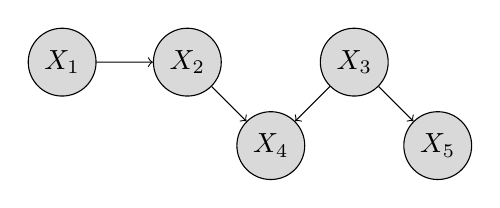
\begin{tikzpicture}[scale=0.53]
\tikzstyle{every node}=[draw,shape=circle,fill=gray!30];
\node (x1) at (0, 2) {$X_1$};
\node (x2) at (3, 2) {$X_2$};
\node (x3) at (7, 2) {$X_3$};
\node (x4) at (5, 0) {$X_4$};
\node (x5) at (9, 0) {$X_5$};
\draw [->]  (x1) -- (x2);
\draw [->]  (x2) -- (x4);
\draw [->]  (x3) -- (x4);
\draw [->]  (x3) -- (x5);
\end{tikzpicture}
\caption{Bayesian network of Example \ref{exBN}}
\label{BN}
\end{center}
\end{figure}
We can encode it in the following PCC agent: 
\begin{lstlisting}[mathescape=true]
joint(X$_1$,...,X$_5$)->
  X$_1$$\sim$ pd$_1$, X$_3$ $\sim$ pd$_4$, 
  (X$_1$=0$\rightarrow$ X$_2$$\sim$ pd$_2$),X$_1$=1$\rightarrow$ X$_2$$\sim$pd$_3$,
  (X$_2$=0,X$_3$=0$\rightarrow$ X$_4$$\sim$pd$_5$),(X$_2$=0,X$_3$=1$\rightarrow$ X$_4$$\sim$pd$_6$),
  (X$_2$=1,X$_3$=0$\rightarrow$ X$_4$$\sim$pd$_7$),(X$_2$=1,X$_3$=1$\rightarrow$ X$_4$$\sim$pd$_8$),
  (X$_3$=0$\rightarrow$ X$_5$$\sim$pd$_9$),(X$_3$=1$\rightarrow$ X$_5$$\sim$pd$_{10}$). 
 \end{lstlisting}
\end{example}

In general, given a Bayesian Network defined on $n$ variables $Var=\{X_1, \ldots, X_n\}$ we can define the following PCC agent:

\begin{lstlisting}[mathescape=true]
joint(X$_1$,...,X$_n$)-> R$_1$,...,R$_{n_I}$,Q$_1$...,Q$_{n_D}$
  \end{lstlisting}
where 
$n_I$ is the number of independent variables in $Var$. $R_i= X \sim pd_X$ where X is the $i$-th independent variable in $Var$ and $pd_X$ corresponds to the probability distribution defined by the BN over the values in the domain of $X$;
$n_D$ is the number of dependent variables in $Var$. Each $Q_i$ is associated to a dependent variable and corresponds to a conjunction of formulas. Given a dependent variable $X$ there is exactly one sub-formula in its conjunction to each assignment of the X's parent nodes. Given the $i$-th dependent variable $X$ with parents $Y_1, \ldots, Y_p \subset Var$ we have thus a sub formula in $Q_i$ for each assignment $a=a_1,\ldots,a_p$ of $Y_1, \ldots, Y_p$ and $Q_i(a)$ is of the form:
\begin{lstlisting}[mathescape=true]
(Y$_1$=a$_1$,...,Y$_p$=a$_p$)-> X$\sim$pd$_X^a$
\end{lstlisting}
where $ pd_X^a$ corresponds to the probability distribution defined by the BN over the values in the domain of $X$ for the assignment of the parents nodes $a$.

\begin{theorem}
Given a BN $\mathcal{B}$ and its PCC translation $\mathcal{P}$ defined over the same set of variables $Var= \{X_1, \ldots, X_n\}$, the probability distribution $pd_{\mathcal{B}}$ over the complete assignments of the variables defined by $\mathcal{B}$ is equal to the probability distribution $pd_{\mathcal{P}}$ over the complete assignments of the variables defined by $\mathcal{P}$.
\end{theorem}
\begin{proof}
Given a complete assignment of the variables $x=x_1,x_2, \ldots, x_n$, its probability in $\mathcal{B}$ will be the product of the probability :
$$\prod_{i \in \{1, \ldots, n\}} \mathbb{P}[X_i =x_i | Pa(X_i)=x\restriction_{Pa(X_i)}] $$ 
where $x\restriction_{Pa(X_i)}$  is the restriction of $x$ on $Pa(X_i) \subset Var$ (the set of parent nodes of $X_i$).

The probability to obtain $x=x_1,x_2, \ldots, x_n$ in $\mathcal{P}$ will be the probability to have a successful execution of the agent:
\lstinline[mathescape=true]{joint(x$_1$,...,x$_n$)}.
We will see that the only possible successful execution is the one that does not violate the input constraints $X_1=x_1, \ldots, X_n=x_n$. Following the definition of the agent, for each independent variables we sample from $X_i\sim pd_{X_i}$ and all the samples bring to a failure with the exception of $X_i=x_i$ that has the probability equals to $\mathbb{P}[X_i =x_i]$. For each dependent variable $X_i$ instead we consider the sub-formula $(Y_1=x\restriction_{Y_1}, \ldots, Y_p=x\restriction_{Y_p}) \rightarrow X_i \sim pd_{X_i}^{a}$ with $a=x \restriction_{Pa(X_i)}$ with $Pa(X_i)=\{Y_1, \ldots, Y_p\}$, because is the only one that satisfy the given constraint over the parents node. In this case we sample from $X_i\sim pd_{X_i}^a$ and all the sample bring to a failure with the exception of $X_i=x_i$ that give a contribution equals to $\mathbb{P}[X_i =x_i|Pa(X_i)=x\restriction_{Pa(X_i)}]$. We have described the only successful execution and it has the same probability as in the corresponding case in the BN $\mathcal{B}$.
 
\end{proof}

%%%%%%%%%%%%%%%%%%%%%%%%%%%%%%%%%%%%%%%%%%%%%%%%%%%

\subsection{Markov Random Fields (MRFs)}


A Markov Random Field (MRF) also called Markov network (MN) is a graphical model defined over a set of $n$ variables. The variables are grouped into cliques $C_1, \ldots , C_k$ each one associated with the joint probability $pd_1, \ldots , pd_k$ defined on the assignments of the variables in that clique. The joint probability of a complete assignment of the variables of the MRF corresponds to the product of the joint probability of its cliques.

Cussens in \cite{SLPcussens2001} has formalised a MRF as a SLP.
We can express the same joint probability over the possible assignments of the set of variables with the following PCC agent:
\begin{lstlisting}[mathescape=true]
joint(X$_1$,...,X$_n$)-> C$_1$$\sim$pd$_1$,...,C$_k$$\sim$pd$_k$, 
	C$_i$=([0,0,..,0])->(X$_1^i$=0,...,X$_{k_i}^i$=0),
	...,
	C$_i$=([1,1,..,1])->(X$_1^i$=1,...,X$_{k_i}^i$=1).
\end{lstlisting}
for all cliques $C_i$ defined over binary  variables $X_1^i$, $\ldots$ , $X{k_i}^i$, with domain $\{0,1\}$. Similarly for the non-binary case.


\begin{theorem}
Given a Markov Random Field $\mathcal{M}$ and its PCC encoding $\mathcal{P}$ defined over the same set of variables $Var= \{X_1, \ldots, X_n\}$, the probability distribution $pd_{\mathcal{M}}$ over the complete assignments of the variables defined by $\mathcal{M}$ is equal to the probability distribution $pd_{\mathcal{P}}$ over the complete assignments of the variables defined by $\mathcal{P}$.
\end{theorem}
It is easy to see that the formulation of MRF is similar to the BNs one. The proof of the above theorem follow the same steps as the proof regarding BNs.


%%%%%%%%%%%%%%%%%%%%%%%%%%%%%%%%%%%%%%%%%%%%%%%%%%%


\subsection{Hidden Markov Models (HMMs)}

 Hidden Markov Models are one of the most popular probabilistic models particularly interesting since is a stochastic extensions of regular grammars \cite{chomsky_book}. A HMM is defined as a series of observed outputs generated by a hidden series of states that are unobserved.
The goal is to model the probability of generating an output observation as a function of the hidden states.

A formalisation of HMM as SLP could be found in \cite{SLPmuggleton96} where SLPs are defined as a direct generalisation of Hidden Markov Models. A similar approach can be found in \cite{SLPcussens2001}.

Formally we consider a HMM over a set of states $s_1, \cdots, s_n$ with transition probability $\mathbb{P}(s_i|s_j)=p_j^i$ and labelled productions $l_1, \cdots, l_m$ with output probability $\mathbb{P}(l_i|s_j)=q_i^j$. We can define an HMM with a clause for each non-terminal state $s$:
\begin{lstlisting}[mathescape=true]
hmm(s$_c$,O) ->
  X $\sim$ s$_1$/p$_1^c$+... +s$_n$/p$_n^c$, 
  X=s$_1$$\rightarrow$ Y$\sim$l$_1$/q$_1^1$+...+l$_m$/q$_m^1$,
  ...,
  X=s$_n$$\rightarrow$ Y$\sim$ l$_1$/q$_1^n$+...+l$_m$/q$_m^n$,
  O=[Y|Out], hmm(X,Out).
\end{lstlisting}
\noindent where $s_c$ corresponds to the current state, $O$ to the current output and the clause for each terminal state $s_t$:
\begin{lstlisting}[mathescape=true]
hmm(s$_t$,O)-> O=[].
\end{lstlisting}

Asking \lstinline[mathescape=true]{hmm(s,Y)-?} we obtain the probability distribution over all the possible sequences $Y$ generated starting from a initial state $s$.


%%%%%%%%%%%%%%%%%%%%%%%%%%%%%%%%%%%%%%%%%%%%%%%%%%%
\subsection{Markov Chains (MCs)}

A discrete-time Markov chain is a sequence of random variables defined over the the same domain: a set of states $s_1, \ldots, s_n$. Each random variable is defined by a probability distribution over the set of states, that corresponds to the probability of moving to next state and it depends only on the present state and not on the previous and future ones. The probability to move from a state $s_i$ to a state $s_j$ is given by the (possibly zero) parameter $p_i^j= \mathbb{P} (s_j |s_i)$, and satisfies the property: $\sum_{j=1}^n p_i^j =1$ .

%The SLP formulation of MCs can be seen as special case of HMMs \cite{SLPmuggleton96,SLPcussens2001}.
%Given a MC defined on $n$ states $s_1, \cdots , s_n$ we represent its SLP formulation explicitly as:
%\begin{lstlisting}[mathescape=true]
%p$_i^0$:  MC(s$_i$, X) :- MC(s$_0$, X).
%...,
%p$_i^{n}$:  MC(s$_i$, X):- MC(s$_n$, X).
%MC(s$_f$,s$_f$).
%\end{lstlisting}
%where $s_f$ are the absorbing states (states with $p_f^f=1$ and $p_f^k=0 ~ \forall k \not=f$).

%The query \lstinline[mathescape=true]{?- MC(s$_0$, X)}
%will produce all the possible final states from an initial state $s_0$.

The PCC formulation is:
\begin{lstlisting}[mathescape=true]
mc(S$_i$,X)->(Y$\sim$s$_0$/p$_i^0$+...+s$_n$/p$_i^{n}$, MC(Y,X)),
mc(s$_f$,X)-> mc(s$_f$,s$_f$).
\end{lstlisting}
The queries \lstinline[mathescape=true]{mc(s$_0$, s$_f$)-?} and \lstinline[mathescape=true]{mc(s$_0$, X)-?} returns respectively the probability to start from the state $s_0$ and arrive in the state $s_f$ and the probability distribution over the set of final states, starting from the state $s_0$.



%%%%%%%%%%%%%%%%%%%%%%%%%%%%%%%%%%%%%%%%%%%%%%%%%%%%

\subsection{Stochastic Context Free Grammars (SCFGs)}
Stochastic Context Free Grammars \cite{SCFG_1,SCFG_2} extend context-free grammars allowing a probabilistic description of production rules, and are defined as a tuple $(\mathcal{W},\mathcal{N},\mathcal{R},\mathcal{P})$
where
$\mathcal{N}$ is the set of non-terminal symbols,
$\mathcal{W}$ is the set of terminal symbols,
$\mathcal{R}$ is the set of production rules of the form $A \rightarrow B_1 \cdots B_m$ where $A \in \mathcal{N}$ and  $B_1 , \cdots , B_m \in  \mathcal{N} \cup \mathcal{W}$ and 
$\mathcal{P}$ is the set of probabilities on production rules.

We consider SCFGs in Chomsky Normal Form (from a SCFG not in normal form we can always recover an equivalent Chomsky Normal Form version \cite{chomsky56}), thus we consider only production rules of the form  $A \rightarrow B_1, B_2$ or  $A \rightarrow C$ where $B_1,B_2 \in \mathcal{N}$ and $C \in \mathcal{W}$.

A formalisation of SCFGs as a SLP program can be found in \cite{SLPmuggleton96} and in \cite{SLPcussens2001}.
In particular Muggleton \cite{SLPmuggleton96} explicitly introduced SLPs as generalisations stochastic context-free grammars.

Given a SCFG in Chomsky Normal Form, each non terminal element $nt_i$ is associated with a probability distribution over the set  $\mathcal{N} \times \mathcal{N} \cup \mathcal{W}$ such that
$nt_i \rightarrow (nt,nt)_j$ with probability $p_i^j$ and $nt_i \rightarrow t_k$ with probability $q_i^k$ and $\sum_j p_i^j + \sum_k q_i^k=1$. We can define the following PCC agent inducing the same probability over the productions:
for the $i$-th non-terminal $N$, we have:
\begin{lstlisting}[mathescape=true]
scfg(O,[N|K],T) ->
  X$\sim$ [nt,nt]$_1$/p$^i_1$+...+[nt,nt]$_n$/p$^i_{n}$+
  t$_1$/q$^i_1$+...+t$_m$/q$^i_m$,
  T=[N|T1],append(X, K, XK),scfg(O,XK,T1).
\end{lstlisting}
for every terminal $d$, we have:
\begin{lstlisting}[mathescape=true]
scfg(O,[d|K],T)->
  O=[d|O1],T=[d|T1],scfg(O1,K,T1).
\end{lstlisting}
and for an empty sequence:
\begin{lstlisting}[mathescape=true]
scfg(O,[],T) -> O=[],T=[].
\end{lstlisting}
where $(nt,nt)_j$ are all the possible pairs of non terminal elements and $t_j$ are all the possible terminal elements.
The first argument of the agent $scfg$ corresponds to the current output string, the second argument to the list of elements to process (terminal or non-terminal), and the last argument corresponds to the parsing tree.

%Since a SCFG provide a probability distribution given a non-terminal over the set of non terminal pairs and terminal elements, the sum of the $p_i$ and $q_j$ terms is equal to one: $$ \sum_{i=1}^n p_i +\sum_{j=1}^m q_j =1 ~ .$$

We can generate sentences using the following query: \lstinline{scfg(O,r,T)-?}. The output will be the probability distribution over all the possible strings $S$ and the corresponding parsing trees $T$, given the non-terminal element corresponding to the root $r$.



%%%%%%%%%%%%%%%%%%%%%%%%%%%%%%%%%%%%%%%%%%%%%%%%%%%
\subsection{Markov Logic networks (MLNs)}
Markov Logic networks \cite{markovLogicNetworks} are defined as a collection of first order logical formulas \(F_j\) (for \(j\in 1\ldots K\)), each associated with a real number \(w_j\), the {\em weight} of the rule. Assume given a set of constants \(\{c_1,\ldots, c_L\}\) (in a 1-1 relationship with intended domain of interpretation), and \(a_1,\ldots, a_N\), an enumeration of the ground atoms (built from the given constants and the predicates in the formulas). Then the joint probability of the network given the truth values \(X_1, \ldots, X_n\) (for the ground atoms \(a_i\)) is given by:
\[ joint(X_1,\ldots, X_n)= (1/Z)\times \prod_{F_j} e^{w_j n_j}
\]
\noindent where \(n_j\) is the number of true groundings of \(F_j\) for the given assignment. \(Z\) is the normalization factor.

We can represent this MLN as a PCC agent \mcode{joint(X1,...,Xn)} using an interpreter for quantifier-free first-order formulas written in CCP (see the agent {\tt v/2}). 
For any formula \(F_i\) let \(F_i^1, \ldots, F_i^{p_i}\) enumerate its \(p_i\) groundings. For any ground formula \(F\), let \([F]\) stand for the formula obtained by replacing each occurrence of \(a_k\) by the variable \(X_k\) (for all \(k\)). 

The predicate \mcode{joint/n} has a single rule with \(n+2\times\Pi_{j\in 1\ldots K} p_j\) atoms in the body. The \(n\) \mcode{b(Xi)} agents each probabilistically guess the value of \mcode{Xi} (drawn from the domain \mcode{\{true,false\}}. Thus computation will result in one probabilistic branch for each of these valuations, each with a probability factor of \(0.5^{n}\) contributed by the \mcode{b/1} agents (hence these factors will get normalized out). The subsquent pairs of agents force a a value for \(\mbox{\tt Y}_{\mbox{\tt i}}^{\mbox{\tt j}}\) (for {\tt i} ranging from {\tt 1} to {\tt K} and for {\tt j} ranging from {\tt 1} to \(\mbox{\tt p}_{\mbox{\tt i}}\) ) by evaluating the formula \(\mbox{\tt [F}_{\mbox{\tt i}}^{\mbox{\tt j}}\mbox{\tt ]}\) (for the given valuation provided by \(\mbox{\tt X}_{\mbox{\tt i}}\)), and contribute a probability factor for this choice. 
\begin{lstlisting}[mathescape=true]
joint(X$_1,\ldots, $X$_n$) ->
  b(X$_1$), ..., b(X$_n$),
  Y$_1^1 \sim $ true/exp(w$_1$)+ false/1, v([F$_1^1$],Y$^1_1$),
  ...,
  Y$_1^{p_1}\sim$ true/exp(w$_1$)+ false/1 , v([F$_1^{p_1}$],Y$_{p_1}^1$),
  ...,
  Y$_K^1\sim$ true/exp(w$_K$)+ false/1,  v([F$_K^1$],Y$_K^1$)
  ...,
  Y$_K^{p_K}\sim$ true/exp(w$_K$)+ false/1,  v([F$_K^{p_k}$],Y$_K^{p_K}$),
	
b(X) -> X$\sim$true/0.5 + false/0.5.
\end{lstlisting}
\noindent Note that the variables \(\mbox{\tt Y}_{\mbox{\tt i}}\) are local to the body (existentially quantified).

The valuation predicate {\tt v/2} is straightforward to define -- it simply evaluates the first argument based on the values of the \(\mbox{\tt X}_{\mbox{\tt i}}\) supplied at the leaves, using standard CCP idioms.
\begin{lstlisting}[mathescape=true]
v(and(A,B),V) -> v(A,VA), v(B,VB), and(VA,VB,V).
v(or(A,B),V) -> v(A,VA), v(B,VB), or(VA,VB,V).
v(not(A),V) -> v(A, VA), not(VA,V).
v(v(X),V) -> X=V.
and(false, \_, Y) -> Y=false.
and(\_, false, Y) -> Y=false.
and(true,true,Y) -> Y=true.
or(true, \_, Y) -> Y=true.
or(\_, true, Y) -> Y=true.
or(false,false,Y) -> Y=false.
not(true,Y) -> Y=false.
not(false,Y)->Y=true.
\end{lstlisting}

\begin{example}\label{ex_mln}
Following the example given by Richardson et al. \cite{markovLogicNetworks}, we consider the following three formulas $F_1$, $F_2$ and $F_3$: \emph{``Smoking causes cancer''} $F_1=\neg sm(X) \vee ca(X)$ with weight $w_1=1.5$; 
\emph{``If two people are friends, either both smoke or neither does''} $F_2 = \neg fr(X, Y) \vee sm(X) \vee \neg sm(Y)$ and $F_3= \neg fr(X, Y) \vee \neg sm(X) \vee sm(Y) $ with weights $w_2=w_3=1.1$.
\begin{figure}[h!]
\centering
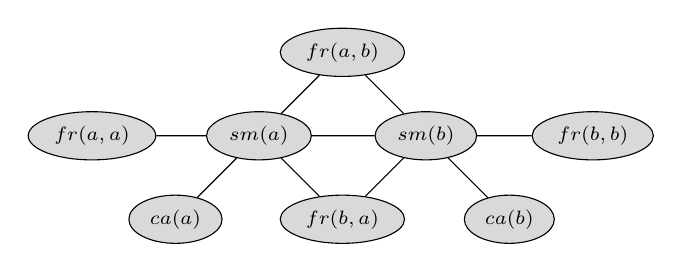
\begin{tikzpicture}[scale=0.53]
\scriptsize
\tikzstyle{every node}=[draw,shape=ellipse,fill=gray!30];
\node (x1) at (0, 2) {$fr(a,a)$};
\node (x2) at (2, 0) {$ca(a)$};
\node (x3) at (4, 2) {$sm(a)$};
\node (x4) at (6, 0) {$fr(b,a)$};
\node (x5) at (6, 4) {$fr(a,b)$};
\node (x6) at (8, 2) {$sm(b)$};
\node (x7) at (10, 0) {$ca(b)$};
\node (x8) at (12, 2) {$fr(b,b)$};
\draw [-]  (x1) -- (x3);
\draw [-]  (x2) -- (x3);
\draw [-]  (x3) -- (x4);
\draw [-]  (x3) -- (x5);
\draw [-]  (x3) -- (x6);
\draw [-]  (x6) -- (x8);
\draw [-]  (x6) -- (x7);
\draw [-]  (x6) -- (x4);
\draw [-]  (x6) -- (x5);
%\coordinate [label=right:$c_1$] (p) at (5.5,2.8);
%\coordinate [label=right:$c_2$] (p) at (5.5,1.3);
%\coordinate [label=right:$c_3$] (p) at (1.6,2.3);
%\coordinate [label=right:$c_4$] (p) at (2.2,1.2);
%\coordinate [label=right:$c_6$] (p) at (8.6,1.2);
%\coordinate [label=right:$c_5$] (p) at (9.3,2.3);
\end{tikzpicture}
\caption{MLN of Example \ref{ex_mln}}
\label{mln}
\end{figure}
In Figure \ref{mln} we can see the graph of the ground Markov network defined by formulas $F_1$, $F_2$ and $F_3$ and the constants \emph{Anna} ($a$) and \emph{Bob} ($b$).


The equivalent PCC agent is defined as follows. Assume the ground atomic formulas are enumerated as:
\lstinline|fr(a,b)|,
\lstinline|fr(a,a)|,
\lstinline|sm(a)|,
\lstinline|sm(b)|,
\lstinline|fr(b,b)|,
\lstinline|ca(a)|,
\lstinline|fr(b,a)| and
\lstinline|ca(b)|. Then we have:
\begin{lstlisting}[mathescape=true]
joint(X$_1$,...,X$_8$) $\rightarrow$ 
  b(X$_1$), ... , b(X$_8$),
  Y$_1^1$$\sim$ true/e$^{w_1}$+ false/1, 
  v(or(not(X$_3$), X$_6$),Y$_1^1$),
  Y$_1^2$$\sim$ true/e$^{w_1}$+ false/1, 
  v(or(not(X$_4$), X$_8$),Y$_1^2$),	
  Y$_2^1$$\sim$ true/e$^{w_2}$+ false/1,
  v(or(not(X$_1$),or(X$_3$, not(X$_4$)),Y$_2^1$),
  Y$_2^2$$\sim$ true/e$^{w_2}$+ false/1,
  v(or(not(X$_2$),or(X$_3$, not(X$_3$)),Y$_2^2$),
  Y$_2^3$$\sim$ true/e$^{w_2}$+ false/1,
  v(or(not(X$_5$),or(X$_4$, not(X$_4$)),Y$_2^3$),
  Y$_2^4$$\sim$ true/e$^{w_2}$+ false/1,
  v( or(not(X$_7$),or(X$_4$, not(X$_3$)),Y$_2^4$),
  Y$_3^1$$\sim$ true/e$^{w_3}$+ false/1,
  v(or(not(X$_1$),or(not(X$_3$), X$_4$)),Y$_3^1$),
  Y$_3^2$$\sim$ true/e$^{w_3}$+ false/1,
  v(or(not(X$_2$),or(not(X$_3$), X$_3$)),Y$_3^2$),
  Y$_3^3$$\sim$ true/e$^{w_3}$+ false/1,
  v(or(not(X$_5$),or(not(X$_4$), X$_4$)),Y$_3^3$),	
  Y$_3^4$$\sim$ true/e$^{w_3}$+ false/1, 
  v(or(not(X$_7$),or(not(X$_4$), X$_3$)),Y$_3^4$).
\end{lstlisting}
\end{example}


It is important to notice that the PCC representation of a MLN has un-normalised weights for its random variables. It is easy to find a normalisation constant that allow to recover the original MLN probability distribution over complete truth assignment of the variables (corresponding to successful executions of the PCC agent) since in the PCC formulation the probability of an execution is the product of the probability over the full set of variables (in each execution we sample all the random variables). So we consider a random variable of the form:
\begin{lstlisting}[mathescape=true]
Y$_i^j$$\sim$ true/e$^{w_i}$+false/e$^0$
\end{lstlisting}
as:
\begin{lstlisting}[mathescape=true]
Y$_i^j$ $\sim$ true/$\frac{e^{w_i}}{e^{w_i}+e^0 }$+false/$\frac{e^0}{e^{w_i}+e^0 }$
\end{lstlisting}
 and at the end of the computation we multiply every execution probability for the following normalisation constant:
 $$Z=\prod_{i=1}^k \prod_{j=1}^{p_i} (e^{w_i} +e^0)=\prod_{i=1}^k (e^{w_i} +e^0)^{p_i}$$






\begin{theorem}
Given a MLN $\mathcal{M}$ defined over a set of clauses $F_j$ and its PCC translation $\mathcal{P}$ 
the probability distribution $pd_{\mathcal{M}}$ defined by $\mathcal{M}$ over the complete truth assignments of the ground atoms  is equal to the probability distribution $pd_{\mathcal{P}}$ defined by $\mathcal{P}$ over the complete truth assignments of the ground atoms.
\end{theorem}
\begin{proof}
Given a input $x_1, \ldots ,x_n$ where $x_1, \ldots , x_n$ are the truth values of the ground atoms $a_1,\ldots, a_n$ generated by the MLN, we want to prove that the probability of $pd_{\mathcal{P}}$ is equal to $pd_{\mathcal{M}}$ on this input. Given the definition of MLN, we have that $pd_{\mathcal{M}}(x_1, \ldots ,x_n)=\prod_{F_j} e^{w_j n_j}$.

Each execution of the PCC agent provide a complete instantiation of the variables $Y_i^j$ by definition of the predicate $jt$. We have thus that the truth value of each grounding formula $[F]_i^j$ is defined: \lstinline[mathescape=true]{v([F]$_i^j$,Y$_i^j$)}. 

The probability of such combination (and the corresponding execution) is the product of the factors associated with each choice: we have a factor $e^{w_i}$ for each \lstinline[mathescape=true]{v([F]$_i^j$,true)} used and $1$ for each \lstinline[mathescape=true]{v([F]$_i^j$,false)} used. Only one of these combinations will succeed, since the input $x_1, \ldots ,x_n$ determines uniquely only one consistent instantiation of the $[F]_i^j$. 
Thus there is only one sampling execution that will succeeds, since every input $x_1,\ldots,x_N$ is consistent with only one instantiation of the $[F]_i^j$.
\end{proof}

%We can define a the same encoding of MLNs in PCCs also in SLPs with minor modifications that we omit due to lack of space. It is important to notice that the SLP formalisation of MLN corresponds to an un-normalised and impure SLP program: un-normalised because the sum of the weights for clauses whose heads share the same predicate could be greater than $1$, and impure since there are rules that don't have a weight.




%%%%%%%%%%%%%%%%%%%%%%%%%%%%%%%%%%%%%%%%%%%%%%%%%%%
%%%%%%%%%%%%%%%%%%%%%%%%%%%%%%%%%%%%%%%%%%%%%%%%%%%
%%%%%%%%%%%%%%%%%%%%%%%%%%%%%%%%%%%%%%%%%%%%%%%%%%%


\section{Conclusion and Future work}
In this paper we have shown the expressiveness of two stochastic approaches for logic programming: Stochastic Logic Programs and Probabilistic Concurrent Constraint Programs.
We have first demonstrated that we can express SLP programs with a PPC agent over discrete random variables, and viceversa for a normalised SLP. We then generalised to un-normalised SLPs.
SLPs and PCCs can express main of the existing probabilistic frameworks. We have shown the direct encoding of some of them in PCC: Bayesian Networks, Markov random fields, Markov chains, Markov Logic networks (also in SLPs), Hidden Markov models and Stochastic Context Free Grammars.
We plan to extend these results to other probabilistic frameworks such as Bayesian logic programs (BLPs)  \cite{LogicBN,LogicBN_1}, Bayesian logic \cite{BLOG}, Problog \cite{ProbLog_original}, etc.
The main future direction is to investigate efficient inference and learning techniques such as ProPPR \cite{proppr_article,proppr_summary,proppr_journal}, FAM \cite{SLPcussens2001} and log-linear models for learning \cite{cussens_1999}. Our goal is to understand the applicability of these parameter estimation techniques to PCC providing efficient inference and learning algorithms.
Another interesting future direction is to show the expressiveness of models that combine probabilistic-logical reasoning  to temporal reasoning: we will focus on the relation between Timed PCC \cite{PCC} and other existing time-based formalisms such as Dynamic Bayesian networks (DBNs) \cite{dynamicBN} and Continuos time Bayesian networks \cite{timeBN}.
We plan also to provide a probabilistic extension of  RCC \cite{RCC} that combines the power of higher-order hereditary Harrop formulas with CCP.


%%%%%%%%%%%%%%%%%%%%%%%%%%%%%%%%%%%%%%%%%%%%%%%%%%%
%%%%%%%%%%%%%%%%%%%%%%%%%%%%%%%%%%%%%%%%%%%%%%%%%%%
%%%%%%%%%%%%%%%%%%%%%%%%%%%%%%%%%%%%%%%%%%%%%%%%%%%
\newpage
\bibliography{bibliographyCORNELIO} 
\bibliographystyle{aaai}
\end{document}
